\documentclass[9pt]{article}
\usepackage[utf8]{inputenc}
\usepackage[margin=0.25in]{geometry}
\usepackage{amsmath}
\usepackage{amsfonts}
\usepackage{amsthm}
\usepackage{hyperref}
\usepackage{multicol}
\usepackage{titlesec}
\usepackage{graphicx}

% documentation: http://ctan.mirror.rafal.ca/macros/latex/contrib/titlesec/titlesec.pdf
\titlespacing*{\section}{0pt}{0ex}{0ex}
\titlespacing*{\subsection}{0pt}{0ex}{0ex}
\titlespacing*{\subsubsection}{0pt}{0ex}{0ex}

\theoremstyle{definition}
\newtheorem{definition}{Definition}[section]
\newtheorem{thm}{Theorem}
\def\xvec{\mathbf{x}}

\begin{document}
\begin{multicols}{2}

% This link gives solutions to Introduction to Statistical Learning (answers in R)
% Just google the title and they can be found
% https://rstudio-pubs-static.s3.amazonaws.com/65566_a44a67a726284943b8f1ec986bf9642d.html

\Large{\textbf{CM763 - Classification Summary}}\\
\normalsize
\begin{definition}[Bias]
Is difference between expected value of dist. of $\hat \theta$ and true, $\text{Bias}(\hat \theta) = E[\hat \theta] - \theta$. Low bias: Trees, $k$-NN, SVM; High bias : LinR, LogR
\end{definition}
\begin{definition}[Prior Distribution]
    $\pi_k = Pr(Y=k)$
\end{definition}
\begin{definition}[Cond. Distrib. of $x$ given $y$]
    $f_{x|y}(X\vert Y=k)= f_k(x)$ (probability density)
\end{definition}
\begin{definition}[Bayes' Rule] 
    $Pr(Y=k\vert X=x) = \frac{Pr(X=x\vert Y=k)Pr(Y=k)}{Pr(X=x)}= \frac{f_k(x)\pi_k}{\sum_{j=1}^k\pi_jf_j(x)}$; $P(A\vert B) = {\displaystyle \frac{P(A)P(B\vert A)}{P(B)}}$
\end{definition}
\begin{definition}[Bayes Classifier]
    $f(x):=\text{argmax}_k Pr(Y=K|X=x)$, or $C(x)=j$ if $P_j(x)=\max\{P_1(x),\dots,P_K(x)\}$. Makes fewest mistakes
\end{definition}
\begin{definition}[Joint Distribution]
    $Pr(X,Y)=Pr(X|Y)Pr(Y)$, $X\in\mathbb{R}^d$
\end{definition}
\begin{definition}[Naive Bayes]
    Assumes $Pr(X|Y) = Pr(X_1|Y)\cdot\Pr(X_2|Y)\dots Pr(X_d|Y)$
\end{definition}
\begin{definition}[Log-odds] 
    $\log\left(\frac{p}{1-p}\right)$
\end{definition}
\begin{definition}[Parametric]
    Can be determined up to finite number of parameters. If finite number of parameters are known, the posterier distribution can be known.  Structure is fixed
\end{definition}
\begin{definition}[Nonparametric]
    Non-deterministic with a finite number of parameters.  If finite number of parameters are known, the posterier distribution still cannot be known.  Can grow without bound as data increases
\end{definition}
\begin{definition}[\href{https://medium.com/@mlengineer/generative-and-discriminative-models-af5637a66a3}{Generative Classifier}]
    Models the distribution of input characteristics of the class (e.g. Naive Bayes Classifier).  A Generative Model learns the joint probability distribution $Pr(x,y)$; it predicts the conditional probability with the help of Bayes Theorem.
\end{definition}
\begin{definition}[\href{https://medium.com/@mlengineer/generative-and-discriminative-models-af5637a66a3}{Discriminant Classifier}]
    Tries to estimate parameters of decision boundary/class separator directly from labelled data. Models $P_k(x)=P(Y=k|X=x)$ directly (e.g. LogR).
\end{definition}
\begin{definition}[Geometric Mean]
    For $n$ numbers, multiply them all together and then take the $n^{\text{th}}$ root: $\sqrt[\leftroot{-2}\uproot{2}n]{a_1 a_2\dots a_n}$
\end{definition}
\textbf{Trade-offs}: (1) Prediction Accuracy vs Interpretability; (2) Good fit vs Underfit/Overfit (3) Parsimony vs Complex. \textbf{Sensitivity}: commonly used to validate the accuracy of a classifier; Predicted True/Total events. \textbf{Selection Bias}: when sample obtained not representative of population
\section{Linear Classifiers}
\subsection{Linear Regression}
[\textit{parametric}] A linear relationship between response and explanatory variables, i.e. $y = \beta_0+\beta_1x+\epsilon$.  If you want to estimate probabilities, use LR.  If $>2$ categories, LinR not appropriate since arbitrary numeric values to categories $\implies$ bigger ``difference'' $\implies$ use Discrim. Analysis
\subsection{Gaussian Classifiers: LDA \& QDA}
Assumes Gaussian distribution for densities, $X|Y=k\sim N_p(\mu_k,\Sigma_k)$.  $f_k(x) = \frac{1}{(2\pi)^{p/2}\vert\Sigma_k\vert^{1/2}}\exp\left(-\frac{1}{2}(x-\mu_k)^T\Sigma_k^{-1}(x-\mu_k)\right)$.  Discr. Analysis models the distribution of $X$ in each class separately, then uses Bayes Thm to obtain $Pr(Y|X)$
\begin{definition}[Discriminant Variables]
    linear combinations of features
\end{definition}
\subsubsection{Linear Discriminant Analysis}
LDA assumes $\Sigma_k$ all equal. Compute discriminant function for each class then classify to largest. $G(x)=\text{argmin}_k\delta_k(x)$ where $\delta_k(x) = \log f_k(x)\pi_k = \log\pi_k-\frac{1}{2}\mu_k^T\Sigma^{-1}\mu_k+x^T\Sigma^{-1}\mu_k$ (discriminant function).   Each discriminant is a linear combination of predictors. $\pi_k$ \& $\mu_k$ can be est. from sample. $\Sigma$ can be estimated by ``pooled variance'': $\hat \Sigma=\frac{(x-\hat \mu)^T(x-\hat \mu)}{n-K}$ \\
\textbf{PCA vs LDA}: PCA (unsupervised) finds axis of maximal variance. LDA finds a feature-space that maximizes class separability
\subsubsection{Quadratic Discriminant Analysis}
QDA does not assume $\Sigma_k$ are equal.
\subsection{Logistic Regression}\label{sect:LogR}
[\textit{discriminative/parametric}] ${\displaystyle p(x) = \frac{e^{\beta_0+\beta\cdot x}}{1+e^{\beta_0+\beta\cdot x}}}$. Equiv. to Logit: $\frac{P_i(x)}{1-P_i(x)}= \beta_0+\beta_1x_1+\dots+\beta_px_p$ (to model categorical variables). Predict binary outcome\\
\textit{Multinomial}: $Pr(Y=k|X)={\displaystyle \frac{e^{\beta_{0k}+\beta_{1k}X_1+\dots+\beta_{pk}X_p}}{\sum_{l=1}^Ke^{\beta_{0l}+\beta_{1l}X_1+\dots+\beta_{pl}X_p}}}$\\
Logistic with $L_1$-Regularization: $Q(\beta_0,\dots,\beta_p)=l(\beta_0,\dots,\beta_p)+\lambda\sum_{j=1}^p|\beta_j|$, w/ $\lambda=\infty \implies$all $\beta_j$'s zero. As $\lambda\downarrow$ from $\infty$, most important $\beta_j$ nonzero first, then second, etc.
\subsection{LASSO: $L_1$ Regularization} 
$\sum_{i=1}^n\left(y_i-\beta_0-\sum x_{ij}\beta_j\right)^2+\lambda\sum_{j=1}^p|\beta_j|$.  Min Opt problem essentially objective w/ $\sum_{j=1}^p|\beta_j|\leq t$ constraint. See Section \ref{sect:LogR} for zeroing $\beta_j$'s
\subsection{Ridge Regression: $L_2$ Regularization} Reduces variance by adding Bias. Performs better when most variables useful.  Tuning parameter $\lambda$. Penalizes slope
\subsection{AIC \& BIC}
Smaller the better.  BIC penalizes complex models more than AIC. BIC asymptotically consistent in model selection. AIC tends to choose more complex as $n\rightarrow\infty$
%\subsection{CV \& the Bootstrap}
%CV Error (mean): 
%${\displaystyle CV_K = \sum_{k=1}^K \frac{n_k}{n}\text{MSE}_k}$ where MSE$_k={\displaystyle \sum_{i\in C_k}\frac{(y_i-\hat y_i)^2}{n_k}}$

\section{Nonparametric Classifiers}
\subsection{$K$-Nearest Neighbors}
[\textit{discriminative}] large $K$: low variance, high bias; smaller $K$: high variance, low bias. Struggles in high dimensions.  Classifies using majority vote among $K$ neighbors
\subsection{Smooth Binomial Regression}
[\textit{nonparmetric}] $\log\left(\frac{P_1(x)}{1-P_1(x)}\right) = f(x_1,\dots,x_p)$, a smooth function (e.g. use splines).  But suffers curse of dim.
\subsection{Kernel Density Classification}
$\hat f(x_0) = \frac{1}{n\lambda}\sum_{i=1}^n K_\lambda(x_0,x_i) = \frac{1}{n\lambda}\sum_{i=1}^n K\left(\frac{x_0-x_i}{\lambda}\right)$
\subsection{Naive Bayes Classifier}
[\textit{Indep. Feature Model}].  Apply a flexible model of the ratio of conditional densities directly. In discriminant analysis:
\[
    \log\left[\frac{P(Y=k|\mathbf{X}=\mathbf{x})}{P(Y=K|\mathbf{X}=\mathbf{x})}\right]
    = \log\frac{\pi_k}{\pi_K} + \log\frac{f_k(\mathbf{x})}{f_K(\mathbf{x})}
\]
Naive Bayes \textit{assumes independence of the $X_j$'s}.  (e.g. assumes $Pr(X|Y) = Pr(X_1|Y)\cdot\Pr(X_2|Y)\dots Pr(X_d|Y)$).  Thus our ratio becomes
${\displaystyle 
    \log\frac{\pi_k}{\pi_K} + \log\frac{f_k(x)}{f_K(x)}  = \log\frac{\pi_k}{\pi_K} + \sum_{j=1}^p\log\frac{f_{kj}(x_j)}{f_{Kj}(x_j)}}$ \\
    ${\displaystyle = \alpha_k + \sum_{j=1}^p h_{kj}(x_j)
}$ \quad
Each $h_{kj}(x_j)$ is a log-ratio of densities for $X_j$ between class $k$ and class $K$.  PCA retains the full information of the space $X$, but re-expresses it as uncorrelated components.  Running PCA before naive Bayes can sometimes \textit{substantially} improve performance.
\subsection{Generalized Additive Model}
A generalized additive model is of the form: $g(E(Y|x)) = \beta_0 + f_1(x_1) + f_2(x_2) + \dots + f_m(x_m)$

It is a generalization of generalized linear model (GLM), which is given by: $g(E(Y|x)) = \beta_0 + \beta_1x_1 + \beta_2x_2 + \dots + \beta_mx_m$
GAMs do not allow for interaction terms.  Use $E(f_j(x_j))$ for identifiability
\section{Tree-based Classifiers}
[\textit{nonparametric}] Find partitions that minimize RSS: $\sum_{j=1}^J \sum_{i\in R_j} (y_i-\hat y_{R_j})^2$, ($R_j$ partitions, $\hat y_{R_j}$ mean response) \\
\textit{Variable Importance}: total amount RSS decreased due to predictor, averaged over all trees.  Trees can model interactions between predictors.  Computationally infeasible to consider all divisions
\subsection{Regression Trees}
\textit{Gini index}: $\sum_{k=1}^Kp_{mk}(1-p_{mk})$ measures total variance across $K$ classes; small value $\implies$ node has predominantly one class. \\\textit{Cross Entropy}: $-\sum_{k=1}^Kp_{mk}\log p_{mk}$
\subsection{Tree Pruning}
\textit{Weakest Link Pruning} minimizes $\sum_{m=1}^{|T|} \sum_{x_i\in R_m} (y_i-\hat y_{R_m})^2 + \alpha\vert T\vert$
\subsection{Bagging}
\begin{definition}[Out-of-Bag Error]
    Use remaining $\sim$1/3 observations to calculate error. If $B$ large, this is leave-one-out CV error ($B$: \# of bs samples). $\text{Err}_{OOB}=\frac{1}{n}\sum^n_{i=1}I(y_i\neq\hat y_{i,OOB})$
\end{definition}
\subsection{Random Forest}
\textit{Decorrelates} the trees. Each split has random selection of $m$ (of full set $p$) predictors. Typically, $m\approx\sqrt{p}$. Cannot overfit.  Adding more trees cannot hurt you.
\subsection{Boosting}
Unlike fitting large decision tree (and potentially overfit), boosting learns slowly.  \textit{Tuning Parameters} $B$: \# of trees; $\lambda$: shrinkage param, learning rate, typically 0.01 or 0.001; \# of splits: depth of tree \\
\subsubsection{AdaBoost}
(1) Forest of stumps, (2) some stumps weighted heavier, by $\alpha_m$, (3) built sequentially.
Weight misclassified obs by factor $\alpha_m=\log\left(\frac{1-\text{err}_m}{\text{err}_m}\right)$ where $\hat G_m(x)$ classifer \& ${\displaystyle \text{err}_m=\frac{\sum_{i=1}^n w_{mi}I(y_i\neq\hat G_m(x_i))}{\sum_i w_{mi}}}$.  Stopping criteria hard to determine.  AdaBoost is equivalent to forward stepwise additive with loss as $L(y,f(x)) = e^{-yf(x)}$\\
Stat. Property: $f^*(x) = \text{argmin}_f E\left[e^{-Yf(x)}\right] = \frac{1}{2}\log\frac{P(Y=1|x)}{P(Y=-1|x)}$\\
Proof:$E(e^{-Yf(x)})=P(Y=1|x)e^{-f(x)}+P(Y=-1|x)e^{f(x)}= \frac{P(Y=1|x)}{P(Y=-1|x)}e^{-f(x)}+e^{f(x)}$. Take deriv. w.r.t. $f(x)$, set to zero: $0=-\frac{P(Y=1|x)}{P(Y=-1|x)}e^{-f(x)}+e^{f(x)}\implies f(x) = \frac{1}{2}\log\frac{P(Y=1|x)}{P(Y=-1|x)}$
\textbf{Gradient Boosting}
\textit{Tuning Param}: \# iters $M$; tree size $J$; shrinkage param $\nu$; 
\textbf{XGBoost}: Optimized for efficiently reduce computing time and allocate an optimal usage of memory resources
\section{\href{https://www.youtube.com/watch?v=LXGaYVXkGtg}{Support Vector Machines}}
[\textit{discriminative/parametric}] A hyperplane: $\beta_0+\beta_1x_1+\dots+\beta_px_p$. If $\beta_0=0$, a subspace.  $(\beta_1,\beta_2,\dots,\beta_p)$: normal vector.  When classes nearly separable, SVM better than LR, also LDA.  For non-separable, using budget $C=0$ implies no budget for violations.

$y_i\left(\omega x_i+b\right)\geq 1$ or $y_i\left(\begin{pmatrix}\omega\ b\end{pmatrix}\cdot\begin{pmatrix}x\\ 1\end{pmatrix}\right)\geq 1$.  Hyperplane: $\omega=\omega_1x_1\dots+\omega_nx_n$.  Width of street: ${\displaystyle M = \frac{1}{\Vert\omega\Vert}}$ (without intercept).  To maximize $M$, 
$\min \frac{1}{2}\Vert\omega\Vert^2$ s.t. $y_i(x_i\omega +b)\geq 1$ for $i=1,\dots,n$. (find Lagrangian, \dots)

\makebox[0pt][l]{%
\begin{minipage}{\textwidth}
    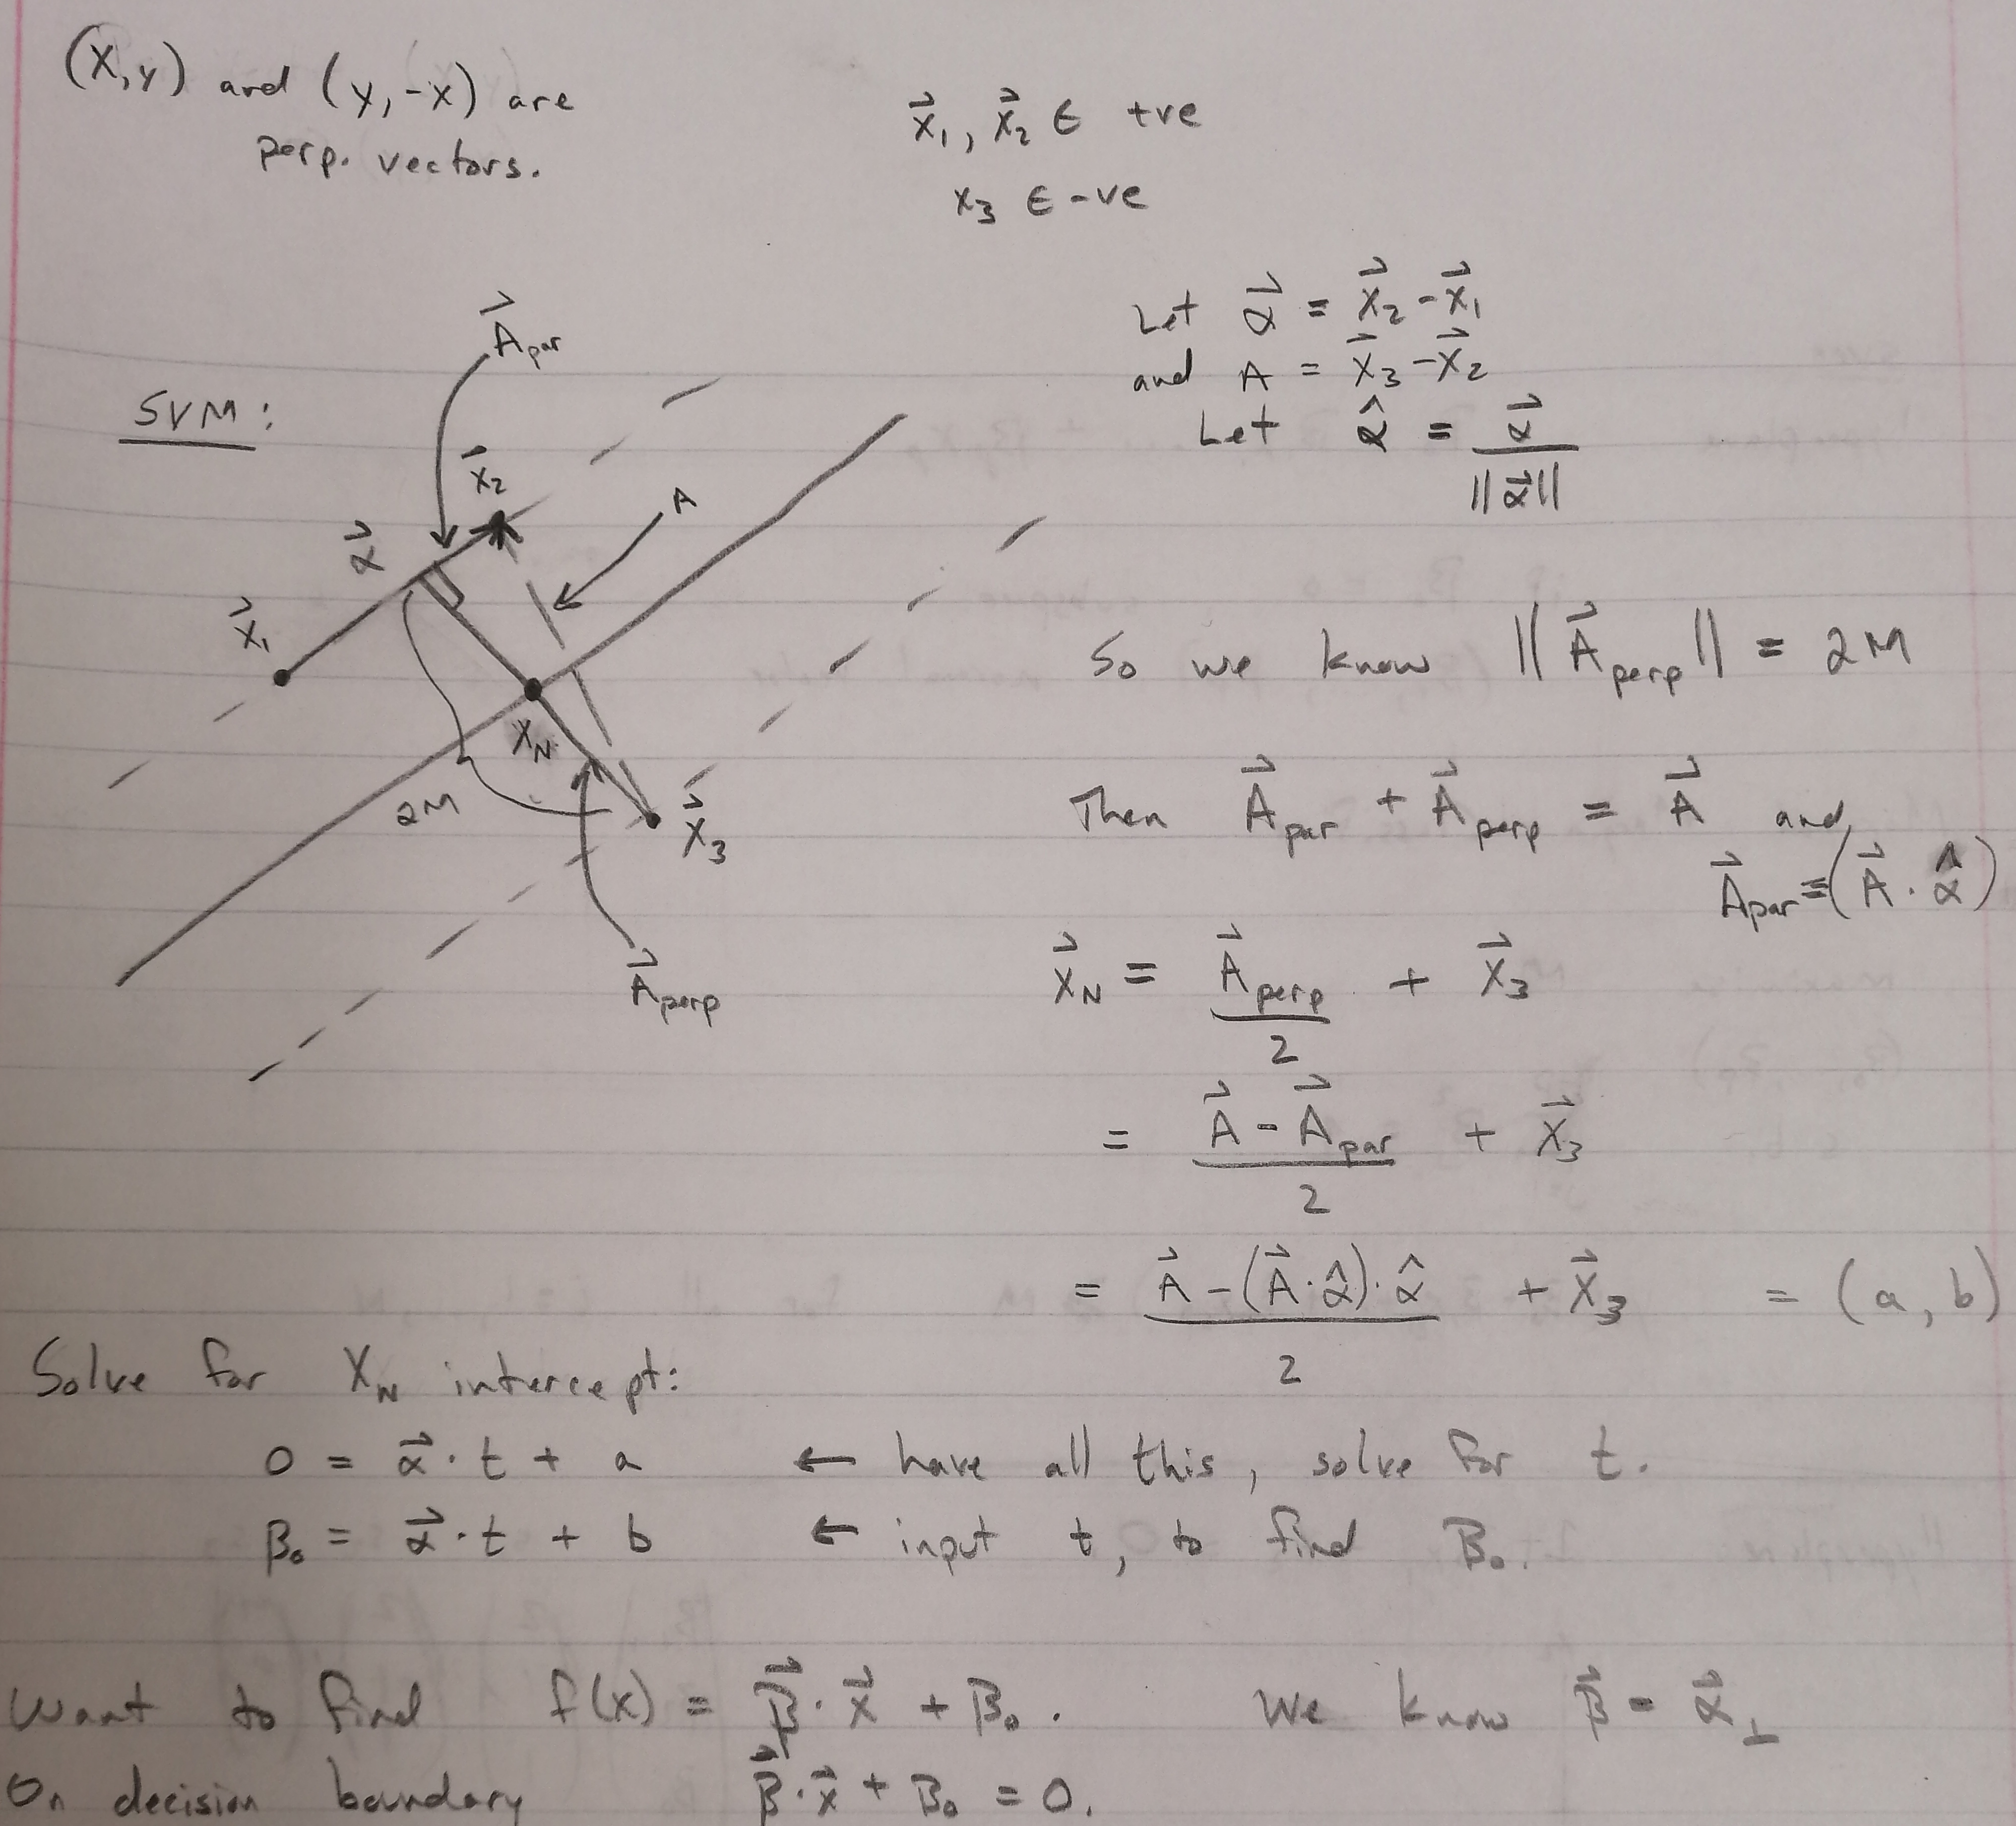
\includegraphics[width=.5\textwidth]{svmsolve.jpg}
 \label{fig:svm}
\end{minipage}
}

\makebox[0pt][l]{%
\begin{minipage}{\textwidth}
    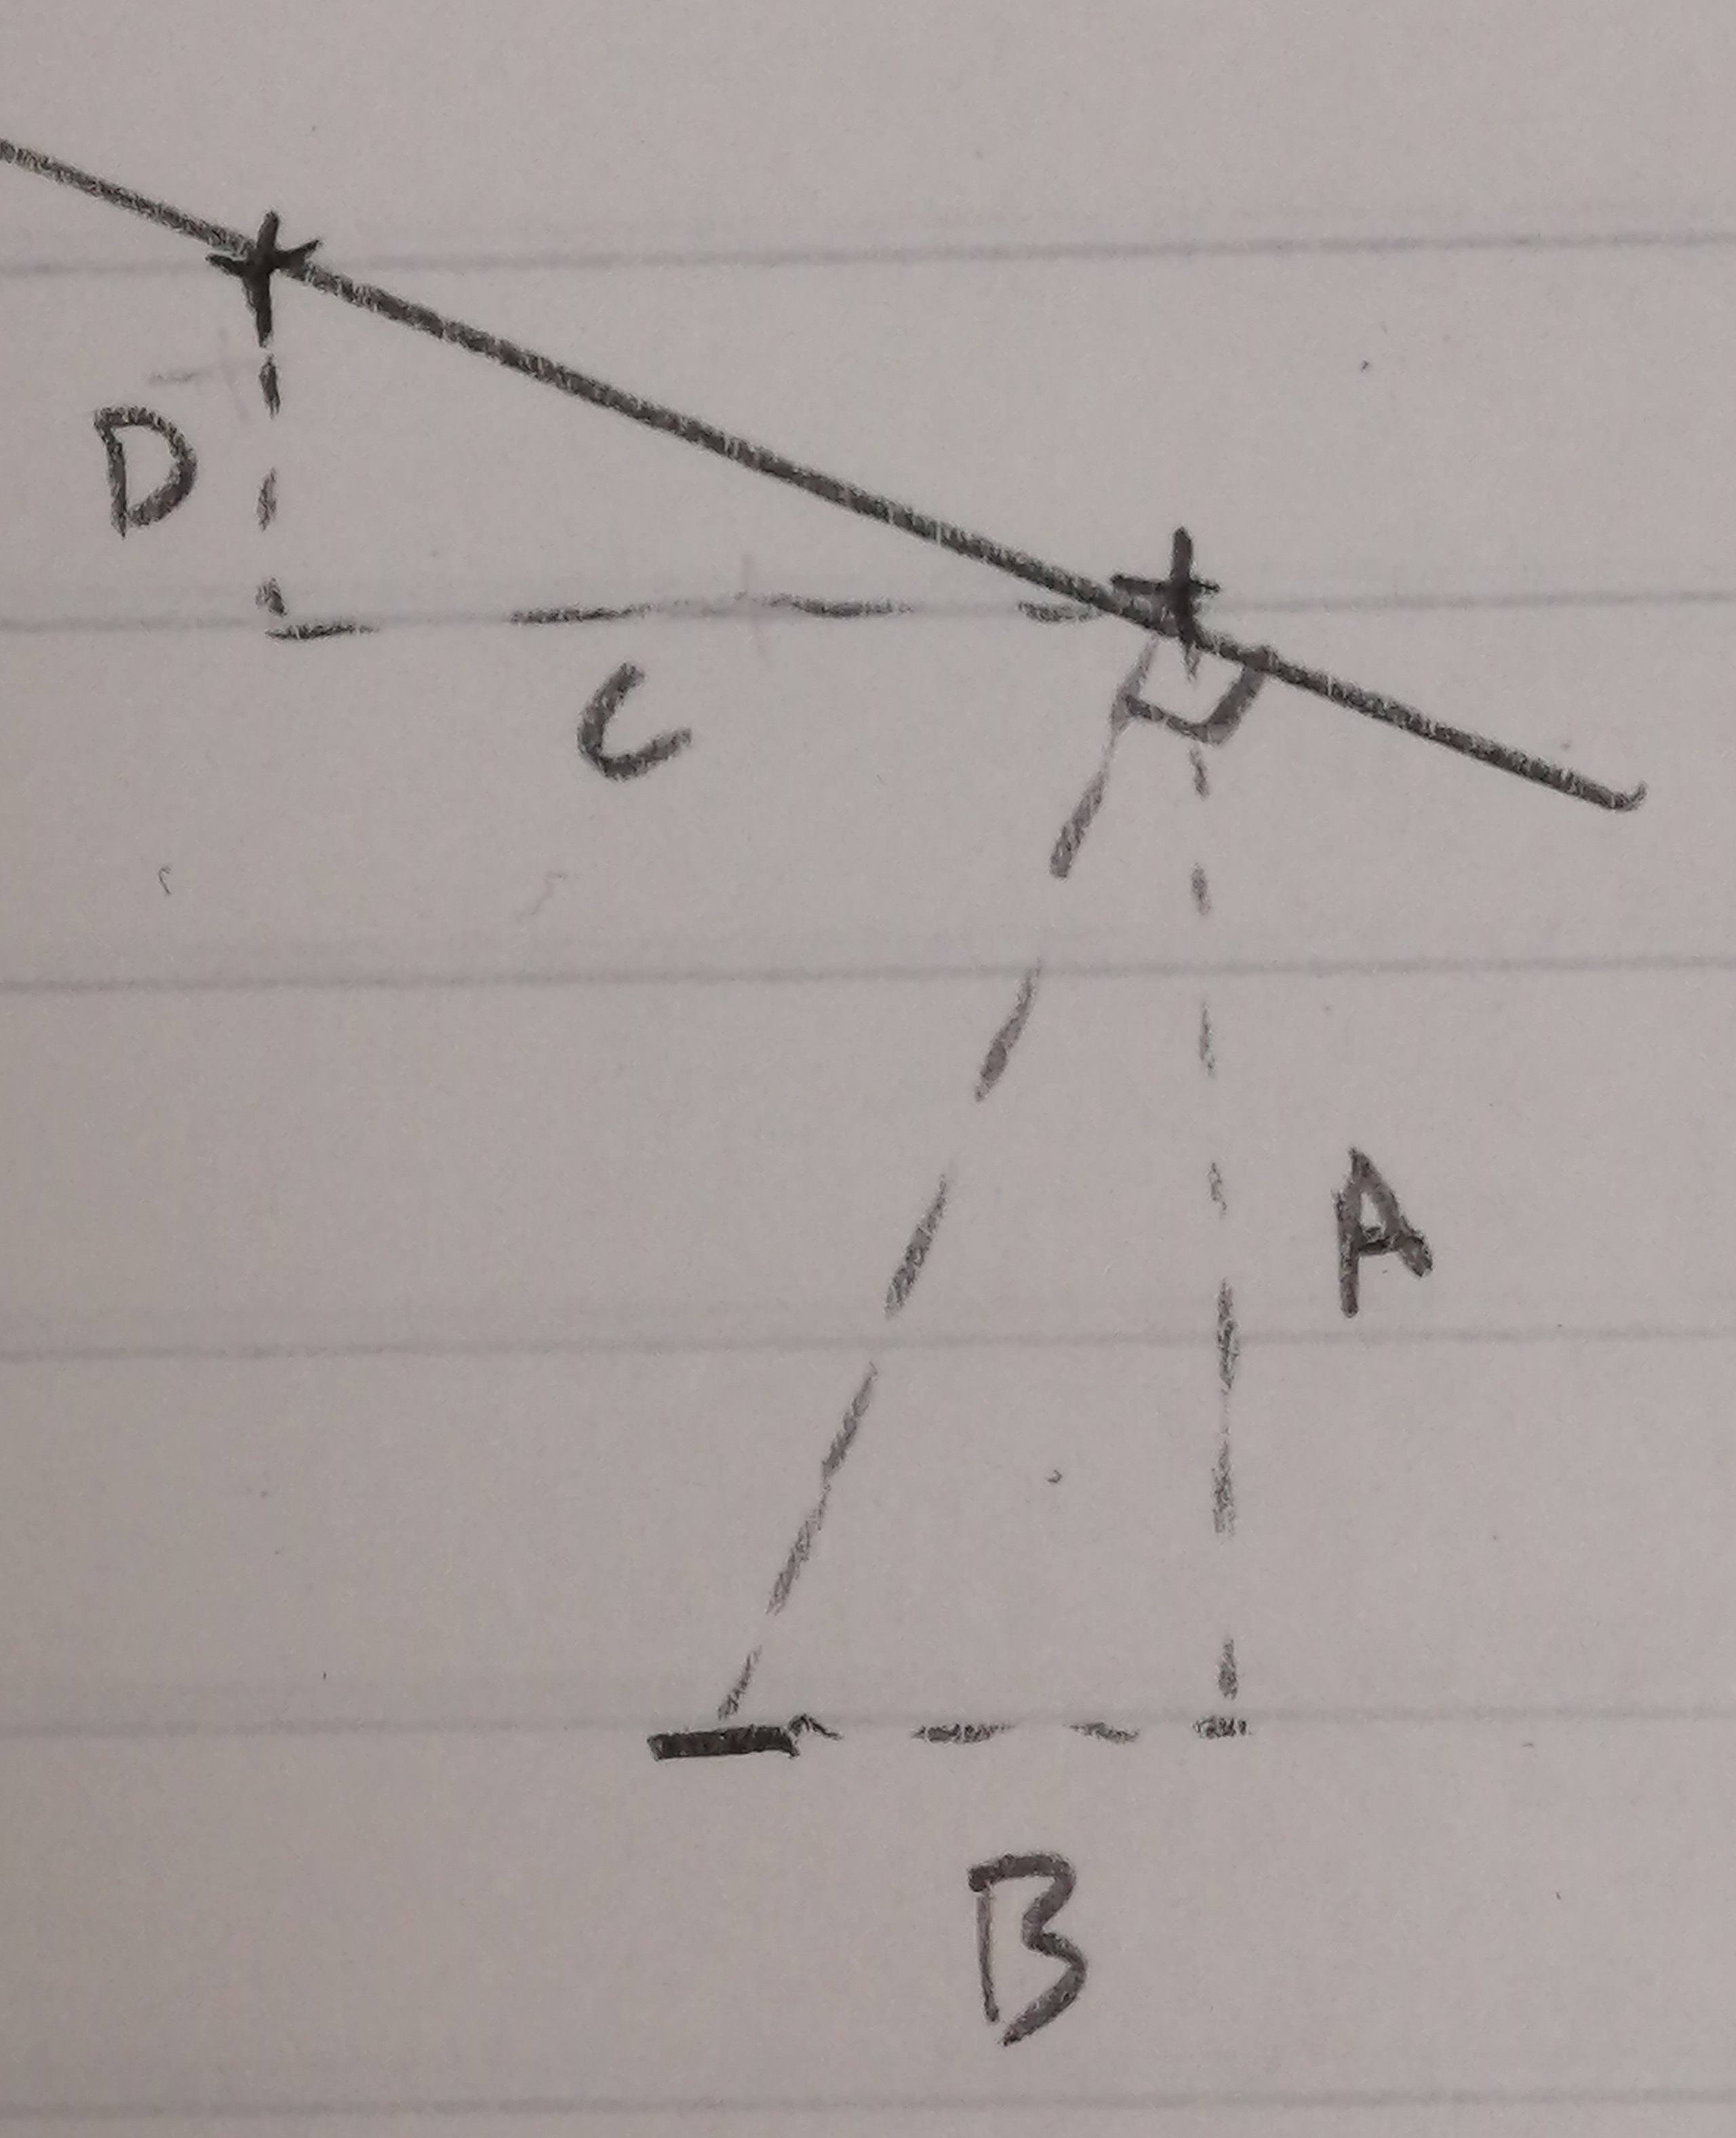
\includegraphics[height=2.5cm]{svmslope.jpg}
 \label{fig:slope}
\end{minipage}
}
\qquad \qquad \qquad \qquad If $\frac{|D|}{|C|}>\frac{|B|}{|A|}$ then use two points.

\subsection{Kernel SVMs}
\subsubsection{Radial Kernel}
[\textit{nonparametric}] $K(x_i,x_{i'}) = \exp\left(-\gamma\sum_{j=1}^p (x_{ij}-x_{i'j})^2\right)$, $\gamma >0$.  It is nonparametric because pairwise distances are calculated between training points, $\gamma$ is determined by CV.  It is a basis expansion, basically the relationship btw 2 pts in $\infty$ dimensions
\subsubsection{$d$-degree Polynomial Kernel}
$K(x_i,x_{i'}) = (1 + \sum_{j=1}^p x_{ij}x_{i'j})^d$. $d$ is usually determined using CV.  A basis expansion in higher dimensions.
\subsection{More than 2 classes}
\subsubsection{One-versus-One}
Constructs $\begin{pmatrix}K\\2\end{pmatrix}$ SVMs. Tally \# of times the obs is assigned to each of $K$ classes. Most frequent class wins
\subsubsection{One-versus-All}
Construct $K$ SVMs, to get $\beta_{0k},\beta_{1k},\dots,\beta_{pk}$ for each $k$. Let $x^*$ be test obs. Classify to $k$, where $\beta_{0k}+\beta_{1k}x^*_k+\dots+\beta_{pk}x^*_p$ largest (most confident)
\textbf{Neural Networks}[\textit{discriminative}]
\end{multicols}
\end{document}
